\documentclass[a4paper,10pt]{article}
\usepackage[utf8]{inputenc}
\usepackage{graphicx}
\usepackage[a4paper]{geometry} %pour les marges
\geometry{hscale=0.77,vscale=0.85,centering}

\title{Configuration de routeur Cisco}
\author{Groupe 1\\Alicia \textsc{Galina}, Corentin \textsc{Ducruet}, Jason \textsc{Bury}, Ishène \textsc{Jemaiel}}
\date{3 octobre 2016}
\begin{document}
\maketitle

\section{Introduction}
En suivant une certaine topologie (figure: \ref{fig:topo}),
nous devions d'abord configurer le routeur qui nous était attribué pour que nous puissions envoyer des pings aux PC des autres membres de notre groupe,
c'est à dire aux PC faisant partie de notre VLAN.
Ensuite, il fallait configurer notre routeur pour pouvoir envoyer des pings aux PC faisant partie d'autres VLAN.
Notre groupe est le groupe 1.

\section{Topologie}
%TODO
\begin{figure}[!h]
 \centering
 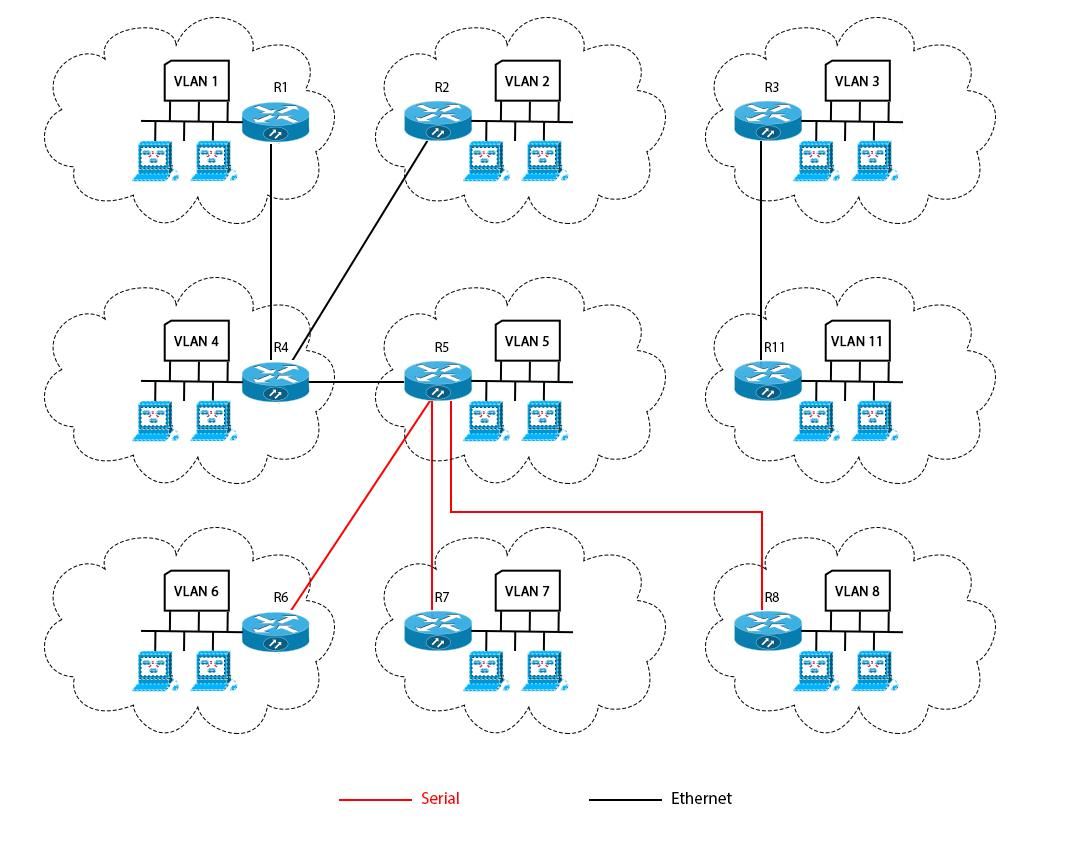
\includegraphics[height=7cm]{topo.jpg}
 \caption{Topologie à suivre pour ce travail pratique}
 \label{fig:topo}
\end{figure}%
Le réseau est composé de 9 VLAN ainsi que 9 routeurs qui sont connectés les uns aux autres (figure: \ref{fig:topo}). Nous avons le routeur R1 (Cisco modèle 2600)qui est connecté au routeur R4.

\section{Configuration}
\subsection{Se connecter}
Une fois connecté au \textit{Secure Console Server} du routeur R1 via l'Access Point sans-fil, Nous accèdons à l'invite de commande du routeur.
La commande suivante nous permet de passer en mode privilégié.
\begin{verbatim}
R1>enable
\end{verbatim}
Notre routeur a deux interfaces:
\begin{itemize}
 \item \textbf{Interface 1/0:} Faisant partie du sous-réseaux contenant notre VLAN.
 \item \textbf{Interface 0/0:} Faisant partie du sous-réseaux contenant R1 et R4 et la connection Point-to-point entre eux.
\end{itemize}

\subsection{Configurer l'interface 1/0}
L'étape suivante consiste donc à configurer l'interface 1/0.
Les IP des réseaux attribués aux groupes sont de la forme 192.168.10$X$.0 où $X$ est le numéro de groupe.
Nous avons choisis d'attribuer à cet interface la plage d'IP correspondant à 192.168.101.0 avec le masque 255.255.255.240.

\textbf{Jusification du masque:} Nous avons 3 PC à connecter à notre VLAN et de plus, il y a 4 ports à notre switch donc nous ne pouvons pas connecter plus de 3 PC à notre routeur.
Nous avons donc besoin d'attribuer une adresse IP de sous-réseaux à 4 noeuds.
Mais l'adresse IP où tous les bits de l'adresse du sous-réseaux sont à 0 est reservée et aussi celle où tous les bits de l'adresse de sous-réseaux est à 1 pour pouvoir effectuer un broadcast.
La plage d'IP doit donc pouvoir contenir 6 adresses et donc le nombre de bits minimum à reserver pour les adresses de sous-réseau est de 3.
Ce qui correspond à un masque de /29.
Mais comme ce masque ne semble pas être accepté par le routeur Cisco, nous avons mis un masque de /28 et là le masque est accepté.
Pour obtenir le masque dans la notation complète, on utilise la notation d'une adresse IP où tous les bits sont à 1 sauf les bits à réserver pour l'adressage du sous-réseaux, qui doivent être les bits de poids le plus faible.
\begin{verbatim}
R1#conf t
R1(config)#int Ethernet1/0
R1(config-if)#ip address 192.168.101.1 255.255.255.240
R1(config-if)#no shutdown
R1(config-if)#exit
R1(config)#exit
R1#sh int
\end{verbatim}
Depuis un PC connecté manuellement à notre VLAN, un ping a été envoyé au routeur avec succès.

\subsection{Service DHCP}
Ensuite nous avons tenté de configurer un serveur DHCP dans le routeur pour notre VLAN.
Remarquez dans notre historique que nous avons exclu l'adresse 192.168.101.1 pour ne pas qu'il soit attribué automatiquement à un de nos PC.
En effet, nous voulons réserver cette adresse pour l'interface du routeur de notre VLAN.
\begin{verbatim}
R1(config)#ip dhcp excluded-address 192.168.101.1 255.255.255.255
R1(config)#ip dhcp pool g1dhcp
R1(dhcp-config)#network 192.168.101.0 255.255.255.240
R1(dhcp-config)#dns-server 192.168.101.1
R1(dhcp-config)#default-router 192.168.101.1
R1(dhcp-config)#lease 1 0 0
R1(dhcp-config)#exit
R1(config)#service dhcp
R1(config)#exit
R1#show ip dhcp server statistics
\end{verbatim}
Le service ne semblait pas opérationnel et la commande affichant les informations sur les adresses IP qui peuvent être attribuées automatiquement ne semble pas fonctionner ou est différente des documentations que nous avons consulté.

\subsection{Service DNS}
%TODO

\subsection{Configurer l'interface 0/0}
Cette fois, avec le groupe 4, nous nous sommes mis d'accord pour utiliser la plage d'adresse 10.11.11.0 avec le masque 255.255.255.248.

Pour le masque, puisque nous avons juste deux routeurs dans ce sous-réseau, il nous faut 2 adresses IP à attribuer en plus des deux adresses qui seront d'office réservées.
Nous aurons donc l'adresse 10.11.11.0 et 10.11.11.3 réservés et nous nous somme mis d'accord pour que le routeur R4 ait l'adresse 10.11.11.1.
L'adresse restante est pour le routeur R1.
\begin{verbatim}
R1#conf t
R1(config)#int Ethernet0/0
R1(config-if)#ip address 10.11.11.2 255.255.255.248
R1(config-if)#no shutdown
R1(config)#exit
R1#sh int
\end{verbatim}
Depuis un PC de connecté à notre VLAN, nous avons pu envoyer un ping au routeur R4.

\section{Service OSPF}
Afin d'obtenir les adresses IP des machines accessibles et connectés au routeur R4, nous avons utilisé le service OSPF.
Dès que nous entrons la commande \texttt{router ospf 1}, le routeur doit recevoir des messages de protocoles OSPF venant du routeur R4.
Le groupe 4 nous avait signalé que le service OSPF du routeur R4 a été configuré. Nous avons tenté de le configuré à notre tour.
\begin{verbatim}
R1(config)#router ospf 1
R1(config-router)#network 192.168.101.0 0.0.0.15 area 1
R1(config-router)#exit
R1(config)#exit
R1#sh ip route
\end{verbatim}
Mais nous observons qu'aucune nouvelle adresse IP a été découverte via le service OSPF.

\end{document}